\documentclass[tikz]{standalone}
\usepackage{physics}
\usepackage{amsmath}
\usepackage{tikz}
\usepackage{mathdots}
\usepackage{yhmath}
\usepackage{cancel}
\usepackage{color}
\usepackage{siunitx}
\usepackage{array}
\usepackage{multirow}
\usepackage{amssymb}
\usepackage{gensymb}
\usepackage{tabularx}
\usepackage{extarrows}
\usepackage{booktabs}
\usetikzlibrary{fadings}
\usetikzlibrary{patterns}
\usetikzlibrary{shadows.blur}
\usetikzlibrary{shapes}
\begin{document}


\tikzset{every picture/.style={line width=0.75pt}} %set default line width to 0.75pt        

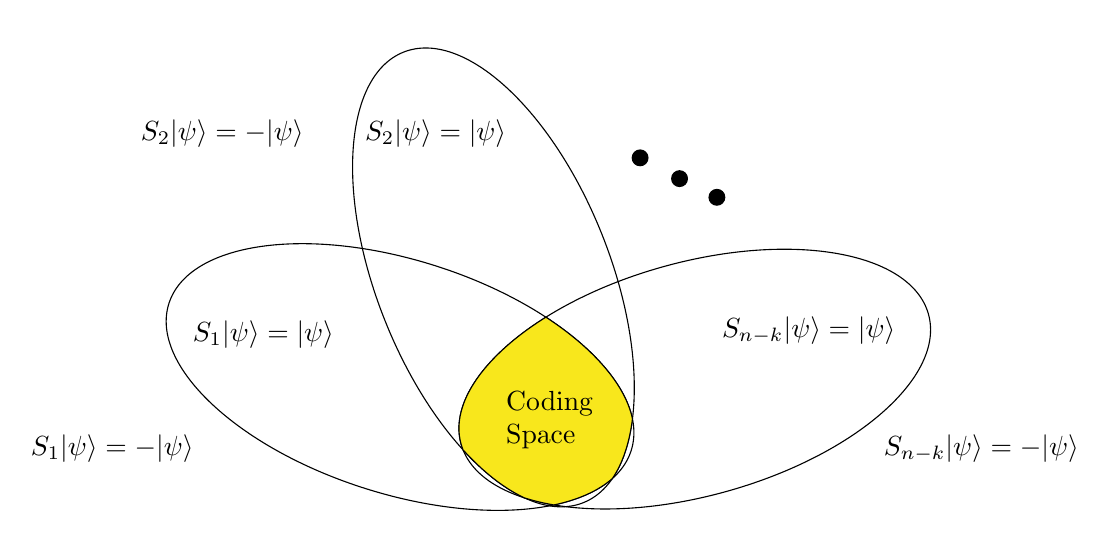
\begin{tikzpicture}[x=0.75pt,y=0.75pt,yscale=-1,xscale=1]
%uncomment if require: \path (0,300); %set diagram left start at 0, and has height of 300

%Shape: Ellipse [id:dp4820534396408521] 
\draw   (244.9,162.24) .. controls (220.97,102.3) and (224.96,44.37) .. (253.81,32.86) .. controls (282.66,21.34) and (325.45,60.6) .. (349.37,120.54) .. controls (373.3,180.48) and (369.31,238.41) .. (340.46,249.92) .. controls (311.61,261.44) and (268.83,222.18) .. (244.9,162.24) -- cycle ;
%Shape: Ellipse [id:dp9793172752168875] 
\draw   (235.09,242.99) .. controls (173.59,223.43) and (131.36,183.58) .. (140.77,153.98) .. controls (150.18,124.37) and (207.67,116.23) .. (269.18,135.79) .. controls (330.68,155.35) and (372.91,195.2) .. (363.5,224.8) .. controls (354.09,254.4) and (296.6,262.55) .. (235.09,242.99) -- cycle ;
%Shape: Ellipse [id:dp7327301805535098] 
\draw   (379.09,136.2) .. controls (441.27,118.93) and (498.42,129.19) .. (506.73,159.12) .. controls (515.05,189.05) and (471.37,227.31) .. (409.18,244.58) .. controls (347,261.85) and (289.85,251.59) .. (281.54,221.66) .. controls (273.22,191.73) and (316.9,153.47) .. (379.09,136.2) -- cycle ;
%Shape: Path Data [id:dp08756783341740537] 
\draw  [fill={rgb, 255:red, 248; green, 231; blue, 28 }  ,fill opacity=1 ] (364.11,209.56) .. controls (362.65,221.19) and (359.4,231.03) .. (354.42,238.3) .. controls (347.71,244.23) and (338.04,248.51) .. (326.28,251.02) .. controls (321.22,250.16) and (316.47,249.02) .. (312.09,247.61) .. controls (302.31,243.08) and (292.19,235.13) .. (282.48,224.46) .. controls (282.12,223.55) and (281.8,222.61) .. (281.54,221.66) .. controls (276.11,202.12) and (292.84,179.03) .. (322.4,160.55) .. controls (345.42,175.57) and (360.74,193.24) .. (364.11,209.56) -- cycle ;
%Shape: Circle [id:dp08592429931812717] 
\draw  [fill={rgb, 255:red, 0; green, 0; blue, 0 }  ,fill opacity=1 ] (364,83.8) .. controls (364,81.7) and (365.7,80) .. (367.8,80) .. controls (369.9,80) and (371.6,81.7) .. (371.6,83.8) .. controls (371.6,85.9) and (369.9,87.6) .. (367.8,87.6) .. controls (365.7,87.6) and (364,85.9) .. (364,83.8) -- cycle ;
%Shape: Circle [id:dp21725683128253837] 
\draw  [fill={rgb, 255:red, 0; green, 0; blue, 0 }  ,fill opacity=1 ] (383,93.8) .. controls (383,91.7) and (384.7,90) .. (386.8,90) .. controls (388.9,90) and (390.6,91.7) .. (390.6,93.8) .. controls (390.6,95.9) and (388.9,97.6) .. (386.8,97.6) .. controls (384.7,97.6) and (383,95.9) .. (383,93.8) -- cycle ;
%Shape: Circle [id:dp9743853567599153] 
\draw  [fill={rgb, 255:red, 0; green, 0; blue, 0 }  ,fill opacity=1 ] (401,102.8) .. controls (401,100.7) and (402.7,99) .. (404.8,99) .. controls (406.9,99) and (408.6,100.7) .. (408.6,102.8) .. controls (408.6,104.9) and (406.9,106.6) .. (404.8,106.6) .. controls (402.7,106.6) and (401,104.9) .. (401,102.8) -- cycle ;

% Text Node
\draw (234,64) node [anchor=north west][inner sep=0.75pt]    {$S_{2} |\psi \rangle =|\psi \rangle $};
% Text Node
\draw (126,64) node [anchor=north west][inner sep=0.75pt]    {$S_{2} |\psi \rangle =-|\psi \rangle $};
% Text Node
\draw (151,161) node [anchor=north west][inner sep=0.75pt]    {$S_{1} |\psi \rangle =|\psi \rangle $};
% Text Node
\draw (73,216) node [anchor=north west][inner sep=0.75pt]    {$S_{1} |\psi \rangle =-|\psi \rangle $};
% Text Node
\draw (406,159) node [anchor=north west][inner sep=0.75pt]    {$S_{n-k} |\psi \rangle =|\psi \rangle $};
% Text Node
\draw (484,216) node [anchor=north west][inner sep=0.75pt]    {$S_{n-k} |\psi \rangle =-|\psi \rangle $};
% Text Node
\draw (302,195) node [anchor=north west][inner sep=0.75pt]   [align=left] {Coding\\Space};


\end{tikzpicture}
\end{document}